\section{NIS,NFS集群}
\begin{figure}[h]
\centering
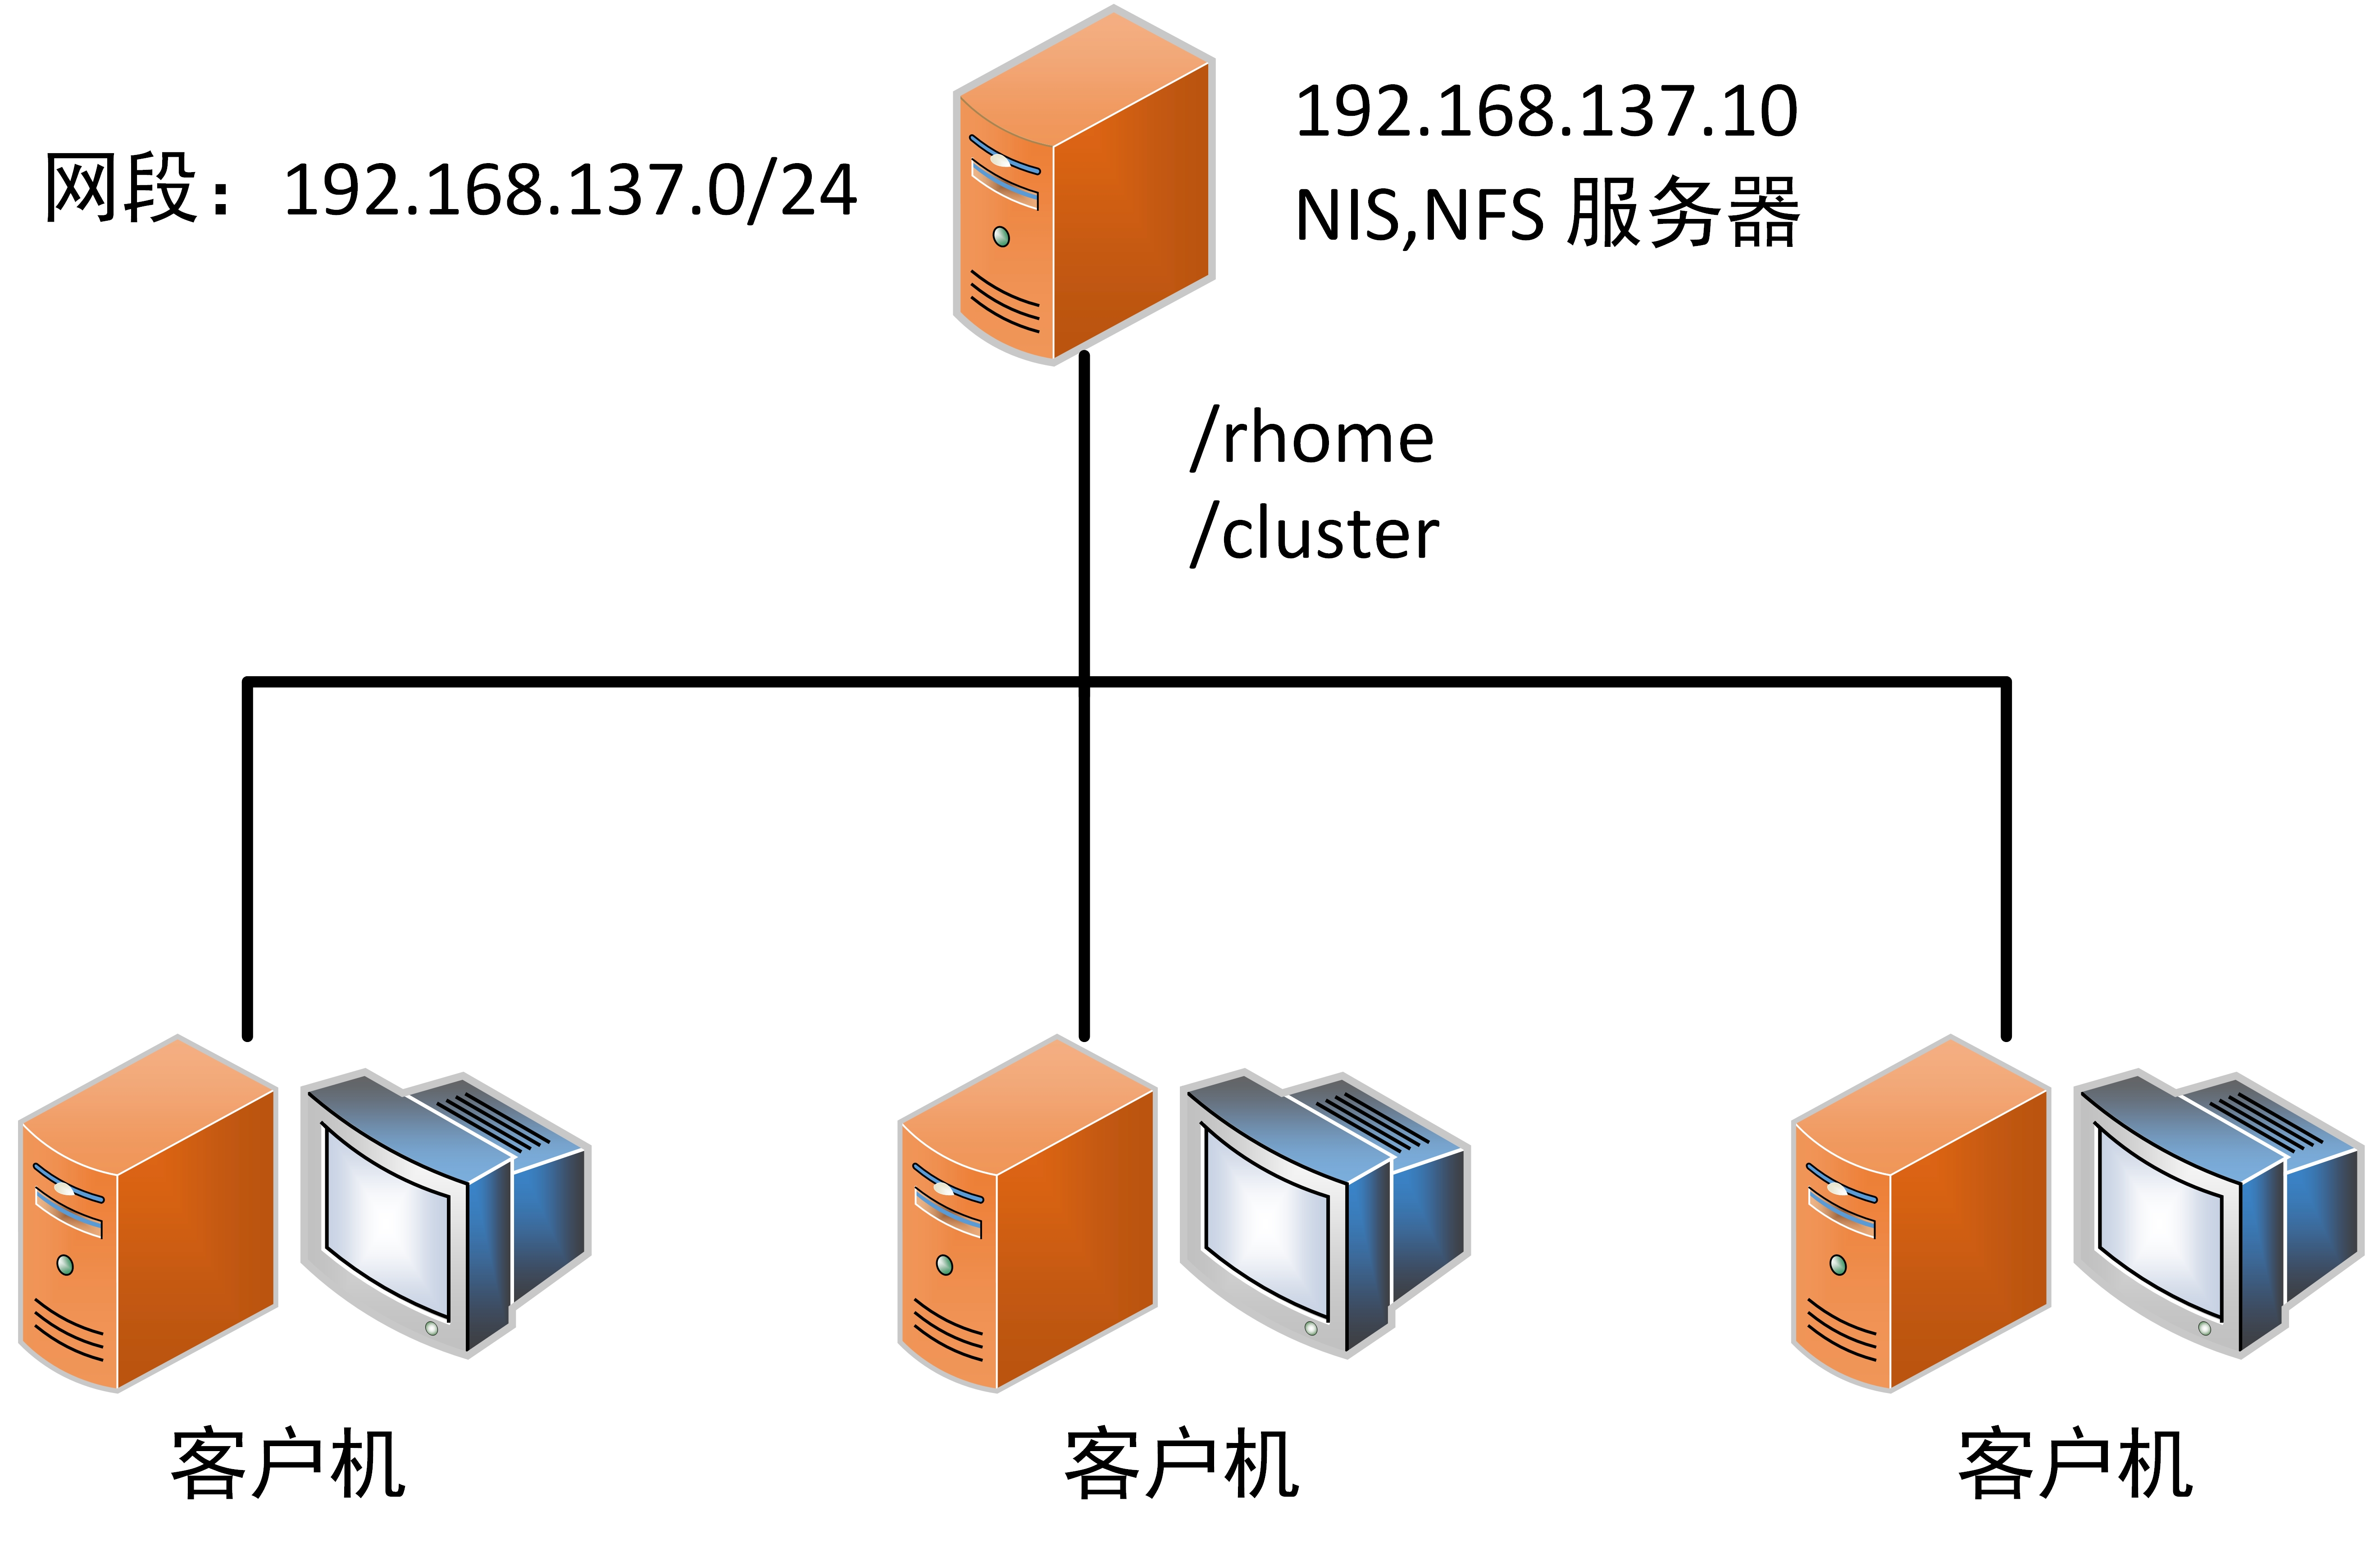
\includegraphics[width=\textwidth]{pic/NIS&NFS.jpg}
\caption{NIS,NFS集群系统}
\end{figure}
建立UID大于2000的账号,账号名为cluser1,cluser2,cluser3, 主目录在/rhome下,新建组clusergroup,将新建的用户加入该组,该组共享文件夹为/cluster. \textbf{目标}:该组人员在任何一台客户机上都能进行自己的工作.

\subsection{配置}
\subsubsection{服务器}
安装: 
\\
\shell{sudo apt-get install nfs-kernel-server nfs-common rpcbind nis -y}
\par
\textbf{1. NIS}
\par
\shell{sudo vim /etc/hosts.deny}
\\\indent 
增加一行:``\texttt{portmap: ALL}".
\par
\shell{sudo vim /etc/hosts.allow}
\\\indent 
增加一行:``\texttt{portmap: 192.168.137.}".
\par
查看本机的主机名并添加到hosts中.
\\
\shell{hostname}\\\indent
或
\\
\shell{cat /etc/hostname}
\par
\shell{sudo vim /etc/hosts}
\\\indent 
增加一行:``\texttt{192.168.137.10   主机名}".
\par
\shell{sudo service rpcbind restart}
\par
\shell{sudo vim /etc/default/nis}
\\\indent 
修改两处:``\texttt{NISSERVER=master}"和``\texttt{NISCLIENT=false}".
\par
\shell{sudo vim /etc/yp.conf}
\\\indent 
添加服务器信息:``\texttt{domain domainName server 主机名}".
\par
domainName就是安装nis时输入的信息,可以直接在 /etc/defaultdomain 中修改,或者运行以下命令修改:
\\
\shell{sudo dpkg-reconfigure nis}
\par
\shell{sudo vim /etc/ypserv.securenets}
\\\indent 
添加客户端所在网段:``\texttt{255.255.255.0   192.168.137.0}".
\par
\shell{sudo vim /var/yp/Makefile}
\\\indent 
修改一行,添加斜体字段:``\texttt{ALL = passwd \textit{shadow} group ...}".
\par
\shell{sudo service ypserv start}
\par
\shell{sudo /usr/lib/yp/ypinit -m}
\par
\shell{sudo service ypserv restart}

\par
\textbf{2. NFS}
\par
\shell{sudo vim /etc/idmapd.conf}
\\\indent 
修改一行:``\texttt{Domain = domainName}".
\par
\shell{sudo vim /etc/default/nfs-common}
\\\indent 
修改一行:``\texttt{NEED\_IDMAPD = YES}".
\par
\shell{sudo service nfs-kernel-server restart}
\par
\shell{sudo service rpcbind restart}

\subsubsection{客户端}
安装:
\\
\shell{sudo apt-get install nfs-common rpcbind nis -y}
\par
\textbf{1. NIS}
\par
\shell{sudo vim /etc/yp.conf}
\par
加入一行:``\texttt{domain domainName server 服务器主机名}".这里的domainName和服务器设置相同.
\par
\shell{sudo vim /etc/nsswitch.conf}
\\\indent
修改几行,添加斜体字段:\\
``\texttt{passwd: compat \textit{nis}}"\\
``\texttt{group: compat \textit{nis}}"\\
``\texttt{shadow: compat \textit{nis}}"\\
``\texttt{hosts: files dns \textit{nis}}"

\par
\textbf{2. NFS}
\par
\shell{sudo vim /etc/hosts.deny}
\\\indent 增加一行:``\texttt{portmap: ALL}".
\par
\shell{sudo vim /etc/hosts.allow}
\\\indent 增加一行:``\texttt{portmap: 192.168.137.10}".
\par
\shell{sudo vim /etc/hosts}
\\\indent 增加一行:``\texttt{192.168.137.10   主机名}".
\par
\shell{sudo vim /etc/idmapd.conf}
\\\indent 修改一行:``\texttt{Domain = domainName}".
\par
\shell{sudo service idmapd restart}
\par
\shell{sudo reboot}

\subsection{搭建}
\subsubsection{服务器}
\par
新建用户并指定主文件夹:\\
\shell{sudo mkdir /rhome}\\
\shell{sudo useradd -u 3001 -d /rhome/cluser1 -m cluser1}\\
\shell{sudo useradd -u 3002 -d /rhome/cluser2 -m cluser2}\\
\shell{sudo useradd -u 3003 -d /rhome/cluser3 -m cluser3}
\par
添加到同一个组:\\
\shell{sudo groupadd clusergroup}\\
\shell{sudo usermod -a -G clusergroup cluser1}\\
\shell{sudo usermod -a -G clusergroup cluser2}\\
\shell{sudo usermod -a -G clusergroup cluser3}
\par
设置该组的公共文件夹,这里要注意的是设置SGID权限:\\
\shell{sudo mkdir /cluster}\\
\shell{sudo chgrp clusergroup /cluster}\\
\shell{sudo chmod 2770 /cluster}
\par
为新建的用户设置密码,并重建YP数据库:\\
\shell{sudo make -C /var/yp}
\par
通过NFS共享到客户端:\\
\shell{sudo vim /etc/exports}
\par
添加两行:\\
``\texttt{/rhome 192.168.137.0/24(rw,no\_root\_squash)}"\\
``\texttt{/cluster 192.168.137.0/24(rw,no\_root\_squash)}"
\par
重启NFS或者重新挂载exports:
\\
\shell{sudo vim exportfs -arv}
\par
验证是否挂载:
\\
\shell{showmount -e localhost}

\subsubsection{客户端}
\par
查看NFS服务器共享情况:
\\
\shell{sudo showmount -e 192.168.137.10}
\par
设置开机挂载:\\
\shell{sudo mkdir /rhome /cluster}\\
\shell{sudo vim /etc/fstab}
\\
\indent 添加两行:\\
``\texttt{192.168.137.10:/rhome /rhome nfs defaults 0 0}"\\
``\texttt{192.168.137.10:/cluster /cluster nfs defaults 0 0}"
\par
\shell{sudo reboot}
\par
接下来,可在客户机上用cluser1等登陆.

